\clearpage
\section{Liturgical Books, Service Items, and Incense}
\PCDPlateHeader{Plate V --- Liturgical Books and Stands}{Relative proportions shown}
\ifdefined\TriptychPrintEdition
\begin{center}
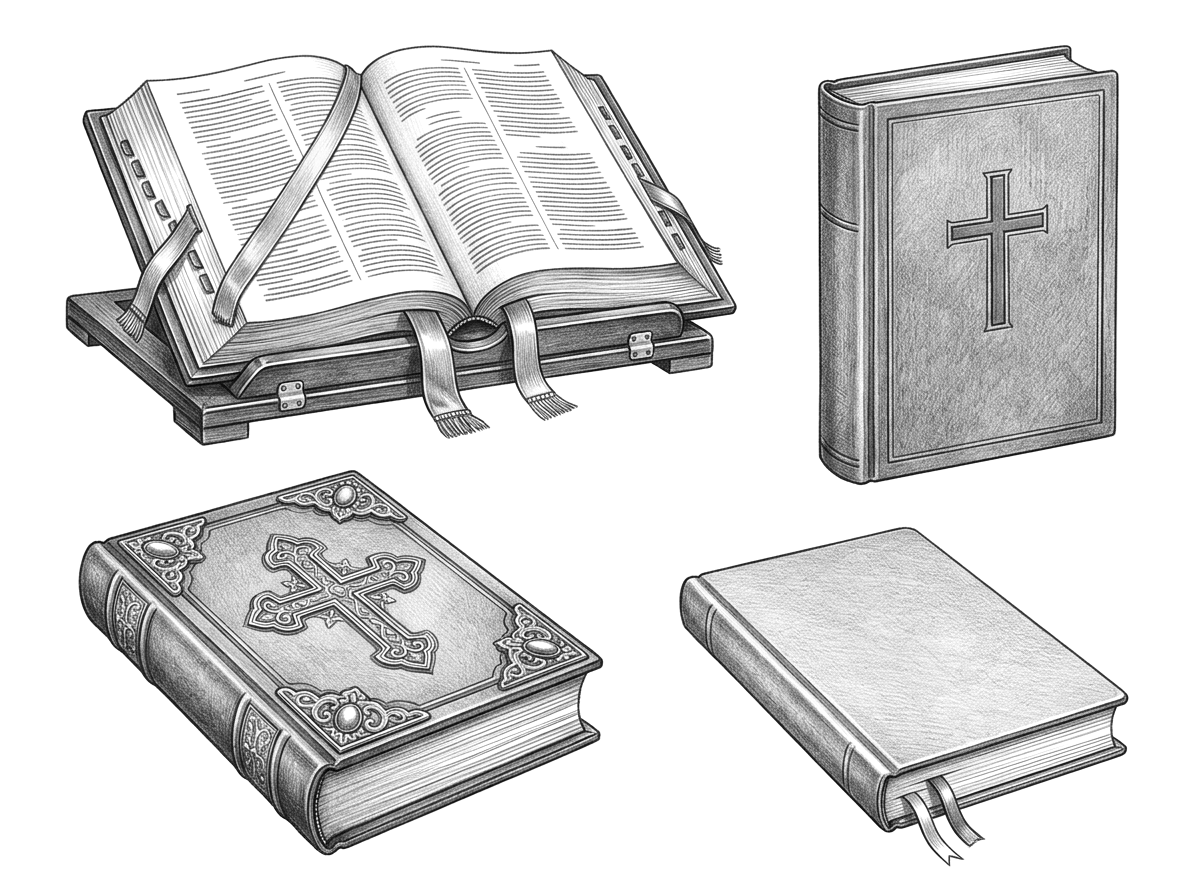
\includegraphics[width=0.92\linewidth,height=3.55in,keepaspectratio]{liturgy/roman-rite/postconciliar/2008-latin-2011-us-english/reference/roman-sanctuary-dictionary/shared/artwork/graphite/pc-art-05-liturgical-books.png}
\end{center}
\PCDPositionKey{Top left: thick Roman Missal open with side tabs and ribbon markers on a low angled Missal Stand; top right: tall closed Lectionary for Mass; bottom left: ornate bound Book of the Gospels (Evangeliary) with metal corner bosses and embossed cross; bottom right: slimmer Book of the Chair (Excerpts from the Roman Missal).}
\else
\textbf{Visual Plate Summary (Plate V --- Liturgical Books and Stands, Relative proportions shown):} Four-book monochrome graphite comparison showing relative scale and binding dignity: top left, a thick altar Roman Missal open flat with ribbon markers and edge tabs on a low angled wooden stand; top right, a tall closed hardcover Lectionary marked with a plain cover cross; bottom left, a heavily ornamented Book of the Gospels with sculpted metal corner bosses and central embossed cross; bottom right, a slimmer handheld Book of the Chair with two ribbon markers.

\textbf{Reading order and object placement:} Top left: thick Roman Missal open with side tabs and ribbon markers on a low angled Missal Stand; top right: tall closed Lectionary for Mass; bottom left: ornate bound Book of the Gospels (Evangeliary) with metal corner bosses and embossed cross; bottom right: slimmer Book of the Chair (Excerpts from the Roman Missal).
\fi

\label{pc-obj-roman-missal}
\PCDEntryHead{Roman Missal}{Missale Romanum}{required}{N20}
\PCDField{Also called}{Altar Missal; Sacramentary (1974--2011 U.S. usage); \textit{Missale}}
Look at top left of Plate V: the Roman Missal is the thick, tabbed ritual book with multiple fringed ribbons resting on the low stand. Before Mass, verify with the priest or sacristan that every ribbon marks the exact page for the day's prayers. When holding the Missal for the priest at the presidential chair, brace the spine firmly with both hands at an easy reading angle without blocking his view; at the Preparation of the Gifts, place it squarely on its stand to the left of the corporal, never touching or covering the corporal.

\PCDField{Where to look on the plate}{Top left, open with edge tabs and ribbons on a low stand (Plate V)}
\PCDField{Handling boundary}{\textbf{Server carries and presents to priest or deacon.} Servers check ribbon markers before Mass as directed, hold the open Roman Missal steady at chest or reading height for the priest at the presidential chair when no stand or Book of the Chair is used, place it cleanly on the altar at the Preparation of the Gifts, and remove it after purification when instructed. (Ordinary ministers: Bishop, Priest.)}
\PCDSafety{Support the heavy altar Missal evenly with both hands or braced cleanly against your upper chest---never by one cover---so the binding does not tear or slip. Never set loose announcements, bulletins, or unapproved sheets atop the Missal or on the altar mensa (GIRM 306).}
\PCDField{Do not confuse with}{Book of the Chair, Lectionary for Mass, Book of the Gospels}
\PCDEntryRule

\label{pc-obj-lectionary}
\PCDEntryHead{Lectionary for Mass}{Lectionarium}{required}{N21}
\PCDField{Also called}{Lectionary; \textit{Ordo lectionum Missae}}
Compare top right and bottom left on Plate V: the Lectionary is the tall hardcover volume with a plain cover cross, distinct from the heavily embossed Book of the Gospels below it. Before Mass, you may help check that the Lectionary is already resting open on the ambo at the exact Sunday (Year A, B, or C) or weekday (Year I or II) reading (GIRM 118b). Remember one firm rule: never carry the Lectionary in the entrance procession (GIRM 120d, 194)---it waits quietly on the ambo before Mass begins.

\PCDField{Where to look on the plate}{Top right, tall closed volume with cover cross (Plate V)}
\PCDField{Handling boundary}{\textbf{Server prepares or sets in place before or during Mass.} Servers may confirm before Mass that the Lectionary lies open to the appointed day's readings on the ambo and may return it to the sacristy after Mass; servers never carry the Lectionary in the entrance procession and never proclaim Scripture from it unless separately deputed as readers. (Ordinary ministers: Bishop, Priest, Deacon, Instituted lector.)}
\PCDSafety{Never carry the Lectionary in the entrance procession---GIRM 120d and 194 strictly reserve the entrance book procession to the Book of the Gospels. Never replace the ritual Lectionary on the ambo with disposable paper leaflets or pew missalettes (GIRM 349).}
\PCDField{Do not confuse with}{Book of the Gospels, Roman Missal}
\PCDEntryRule

\label{pc-obj-book-of-the-gospels}
\PCDEntryHead{Book of the Gospels}{Evangeliarium}{provided}{N22}
\PCDField{Also called}{Evangeliary; Gospel Book; \textit{Liber Evangeliorum}}
Look at bottom left of Plate V: the Book of the Gospels is unmistakably recognized by its heavy embossed cover, central cross in relief, and sculpted metal corner bosses. Keep this liturgical boundary clear: as an altar server, you never carry the Book of the Gospels in the entrance procession (that office belongs to the deacon, or to the lector if no deacon is present: GIRM 120d, 194) and never lift it off the altar before the Gospel. Your privilege is to escort the Gospel procession with lighted candles and the smoking thurible and stand attentively flanking the ambo while the Gospel is proclaimed (GIRM 133, 175).

\PCDField{Where to look on the plate}{Bottom left, ornate metal-bossed cover (Plate V)}
\PCDField{Handling boundary}{\textbf{Server recognizes only; does not handle.} Altar servers never carry the Book of the Gospels in the entrance procession (reserved strictly to the deacon, or to an instituted or deputed lector if no deacon is present) and never lift it from the altar for the Gospel procession; servers escort it with lighted candles and the thurible, flank the ambo during proclamation, and may reverently return the closed volume to the sacristy after Mass. (Ordinary ministers: Bishop, Priest, Deacon, Instituted lector.)}
\PCDSafety{Never hand the Book of the Gospels to an altar server to carry in the entrance procession---GIRM 120d and 194 reserve that role strictly to the deacon or, in his absence, a lector. During the Gospel procession, candle-bearers hold flames well clear of the ornate cover and open pages.}
\PCDField{Do not confuse with}{Lectionary for Mass, Roman Missal}
\PCDEntryRule

\label{pc-obj-book-of-the-chair}
\PCDEntryHead{Book of the Chair}{Excerpts from the Roman Missal (no Latin typical edition)}{territorial adaptation}{N23}
\PCDField{Also called}{Excerpts from the Roman Missal; Presidential Prayer Book}
This slimmer ceremonial book at bottom right of Plate V was created with altar servers in mind. Because the full altar Roman Missal is heavy to hold steadily for long prayers, the Book of the Chair (officially Excerpts from the Roman Missal) contains only the prayers spoken at the presidential chair and entrance. Before Mass, confirm that both ribbons mark the Collect and Prayer after Communion; step promptly before the priest when he rises for prayer, hold the book open flat at a comfortable height without tipping the pages, and return it beside the chair---never to the altar.

\PCDField{Where to look on the plate}{Bottom right, slimmer handheld ceremonial volume (Plate V)}
\PCDField{Handling boundary}{\textbf{Server carries and presents to priest or deacon.} Servers hold the Book of the Chair open flat and steady at the priest's reading angle during the Introductory Rites, Collect, Universal Prayer conclusion, Prayer after Communion, and Final Blessing, and never place it on the altar in place of the complete Roman Missal. (Ordinary ministers: Bishop, Priest.)}
\PCDSafety{Never carry the Book of the Chair to the altar for the Liturgy of the Eucharist or the Eucharistic Prayer---it does not contain the Order of Mass altar prayers or Eucharistic Prayers, which require the complete Roman Missal (GIRM 306).}
\PCDField{Do not confuse with}{Roman Missal, Lectionary for Mass}
\PCDEntryRule

\label{pc-obj-missal-stand}
\PCDEntryHead{Missal Stand}{Pulpitum}{customary}{N24}
\PCDField{Also called}{Altar bookstand; Missal cushion; \textit{Legile}; \textit{Cussinus}}
Look directly beneath the open Roman Missal at top left of Plate V to see the low angled Missal stand. Keep the stand on the credence table---never sitting empty on the bare altar---until the Preparation of the Gifts (GIRM 139, 306). When you carry it to the altar, double-check that its folding hinge is locked securely, set it squarely to the left of the unfolded corporal without touching the linen or edging toward a candle, and remove it neatly after purification when directed.

\PCDField{Where to look on the plate}{Top left, low angled stand beneath the open Missal (Plate V)}
\PCDField{Handling boundary}{\textbf{Server handles directly.} Servers keep the Missal stand off the altar mensa before the Preparation of the Gifts, carry it to the altar alongside the Roman Missal at the Preparation of the Gifts, set it neatly to the left of the corporal without overlapping the linen, and remove it cleanly after purification or Mass. (Ordinary ministers: Bishop, Priest.)}
\PCDSafety{Verify that hinged wooden or metal stands lock firmly at a low angle before setting the heavy Roman Missal upon them so the stand cannot collapse during the Eucharistic Prayer, and never set any edge of the stand over the unfolded corporal.}
\PCDField{Do not confuse with}{Ambo}
\PCDEntryRule

\clearpage
\subsection{Processional and Service Equipment}
\PCDPlateHeader{Plate VI --- Processional and Service Equipment}{Not to common scale}
\ifdefined\TriptychPrintEdition
\begin{center}
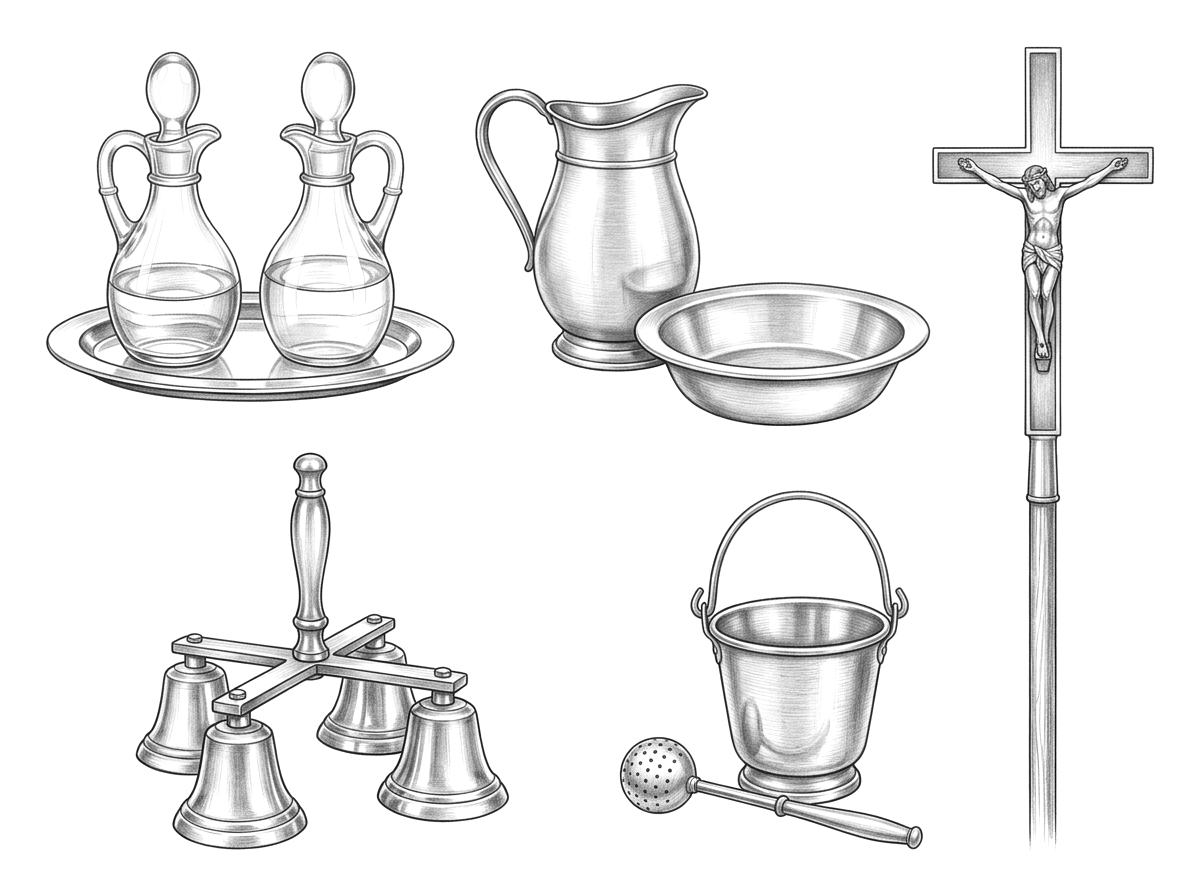
\includegraphics[width=0.92\linewidth,height=3.55in,keepaspectratio]{liturgy/roman-rite/postconciliar/2008-latin-2011-us-english/reference/roman-sanctuary-dictionary/shared/artwork/graphite/pc-art-06-service-cruets-bells.png}
\end{center}
\PCDPositionKey{Top left: paired glass wine and water Cruets with stoppers on a tray; top center: Lavabo pitcher and shallow finger basin; top right: Processional Cross bearing the sculpted corpus of Christ on a staff; bottom left: four-cup mounted brass Sanctuary Bell; bottom right: holy-water Aspersorium bucket and perforated metal Aspergillum.}
\else
\textbf{Visual Plate Summary (Plate VI --- Processional and Service Equipment, Not to common scale):} Five-object monochrome graphite service equipment study: top left, two stoppered transparent glass cruets for wine and water resting on an oval metal tray; top center, a metal lavabo pitcher beside a shallow round finger basin; top right, a tall processional cross on a wooden staff bearing the sculpted figure of Christ crucified; bottom left, a traditional four-bell mounted brass sanctuary hand bell; bottom right, a metal holy-water aspersorium bucket with bail handle and perforated spherical-head aspergillum resting beside it.

\textbf{Reading order and object placement:} Top left: paired glass wine and water Cruets with stoppers on a tray; top center: Lavabo pitcher and shallow finger basin; top right: Processional Cross bearing the sculpted corpus of Christ on a staff; bottom left: four-cup mounted brass Sanctuary Bell; bottom right: holy-water Aspersorium bucket and perforated metal Aspergillum.
\fi

\label{pc-obj-processional-cross}
\PCDEntryHead{Processional Cross}{Crux processionalis}{required}{N25}
\PCDField{Also called}{Altar Cross; Crucifix; \textit{Crux cum figura Christi crucifixi}}
As cross-bearer (crucifer), hold the staff upright with both hands at a steady height so the sculpted figure of Christ faces forward as you lead the ministers behind the thurifer. Never bow or genuflect while carrying the cross (GIRM 274). Once you reach the sanctuary, seat the staff firmly in its floor stand near the altar---or put it away cleanly if a separate altar crucifix is already stationed on or beside the altar (GIRM 122).

\PCDField{Where to look on the plate}{Top right, bearing sculpted corpus on wooden staff (Plate VI); altar cross at center (Plate I)}
\PCDField{Handling boundary}{\textbf{Server carries in procession or movement.} The cross-bearer carries the processional cross upright with the figure of Christ facing forward, omits bowing and genuflecting while holding it (GIRM 274), and sets it securely in its floor stand near the altar or puts it away if another altar cross already stands there (GIRM 122). (Ordinary ministers: Instituted acolyte, Altar server.)}
\PCDSafety{Do not bow or genuflect while holding the processional cross (GIRM 274), both to honor the rubric and to prevent the tall staff from pitching forward. Keep the staff clear of low doorways and hanging lights, and confirm that its weighted floor stand is level and stable before releasing it.}
\PCDEntryRule

\label{pc-obj-altar-candles}
\PCDEntryHead{Altar Candles}{Candelabra cum cereis}{required}{N26}
\PCDField{Also called}{Altar Candlesticks; Processional Candles; \textit{Cerei}; \textit{Candelabra}}
Light the altar candles before Mass with a lighting taper and extinguish them afterward with a snuffer---never blow them out across the white linen cloth. When carrying a candle beside the processional cross or flanking the ambo for the Gospel, hold your candlestick upright at the same height as your partner's, omit bows and genuflects while holding it (GIRM 274), and keep the open flame safely away from hair, sleeves, and books.

\PCDField{Where to look on the plate}{See Plate I, flanking the freestanding altar}
\PCDField{Handling boundary}{\textbf{Server handles directly.} Servers light altar candles shortly before Mass, extinguish them cleanly with a snuffer afterward, and carry processional and Gospel candles upright at matching heights without bowing or genuflecting while holding them (GIRM 120b, 133, 274). (Ordinary ministers: Instituted acolyte, Altar server.)}
\PCDSafety{Keep open flames well clear of hair, albs, ribbons, vestments, and the pages of the Roman Missal. Carry processional candles strictly upright, watch for dripping hot wax, and extinguish every flame with a brass snuffer rather than blowing melted wax onto the white altar cloth.}
\PCDField{Do not confuse with}{Sanctuary Lamp}
\PCDEntryRule

\label{pc-obj-sanctuary-bells}
\PCDEntryHead{Sanctuary Bells}{Campanula}{optional}{N27}
\PCDField{Also called}{Altar Bell; Sanctus Bell; \textit{Parva campanula}}
Place the bell quietly beside your kneeling spot before the Eucharistic Prayer so you never have to reach across the sanctuary during the Canon. Following your parish's custom under GIRM 150, give one brief, clear ring when the priest spreads his hands over the bread and wine at the epiclesis, and ring clearly as he elevates the Host and again as he elevates the Chalice. Damp the bell rims softly against your hand or the carpet when setting it down so the clappers do not jingle.

\PCDField{Where to look on the plate}{Bottom left, four-cup mounted brass altar bell (Plate VI)}
\PCDField{Handling boundary}{\textbf{Server handles directly.} An altar server rings the sanctuary bell cleanly and reverently shortly before the consecration and at each elevation according to local parish custom (GIRM 150), setting it down quietly without rattling the cups. (Ordinary ministers: Altar server, Instituted acolyte.)}
\PCDEntryRule

\label{pc-obj-aspergillum-aspersorium}
\PCDEntryHead{Aspergillum and Aspersorium}{Aspergillum et aspersorium}{optional}{N28}
\PCDField{Also called}{Holy-Water Sprinkler and Bucket; Holy-Water Vessel; \textit{Vas aquae benedicendae}; \textit{Vas aquae benedictae}}
Before a Sunday sprinkling rite, confirm that the clean holy-water bucket is filled roughly two-thirds full on the credence table with the sprinkler beside it (GIRM 118c). Bring both to the priest at the chair or altar when signaled, hand him the sprinkler handle first, and walk steadily at his side through the aisle holding the bucket level so he can dip easily without spilling water on the steps. Return both pieces to the credence table as soon as the sprinkling ends.

\PCDField{Where to look on the plate}{Bottom right, holy-water bucket and perforated sprinkler (Plate VI)}
\PCDField{Handling boundary}{\textbf{Server carries and presents to priest or deacon.} Servers fill the clean vessel on the credence table before Mass, bring it to the priest for the blessing and sprinkling rite, accompany him through the nave holding the bucket steady, and return both articles cleanly to the credence table afterward (GIRM 51, 118c). (Ordinary ministers: Bishop, Priest, Deacon.)}
\PCDSafety{Fill the bucket only half to two-thirds full so water does not slosh over the rim onto stone or polished sanctuary steps and create a slipping hazard for ministers and communicants.}
\PCDField{Do not confuse with}{Cruets, Baptismal Font}
\PCDEntryRule

\clearpage
\subsection{Thurible, Charcoal, and Incense Boat}
\PCDPlateHeader{Plate VII --- Incense Equipment}{Not to common scale}
\ifdefined\TriptychPrintEdition
\begin{center}
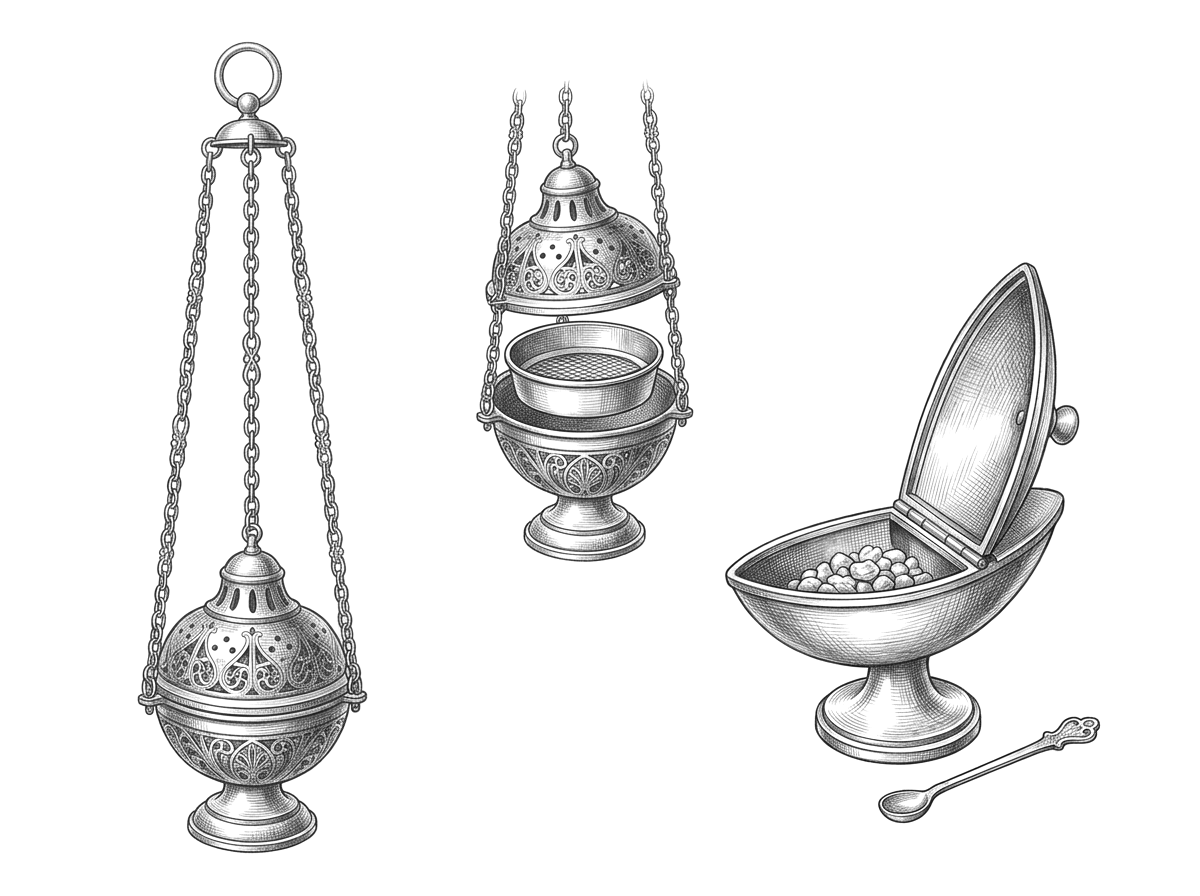
\includegraphics[width=0.92\linewidth,height=3.55in,keepaspectratio]{liturgy/roman-rite/postconciliar/2008-latin-2011-us-english/reference/roman-sanctuary-dictionary/shared/artwork/graphite/pc-art-07-incense-set.png}
\end{center}
\PCDPositionKey{Left: closed metal Thurible suspended on outer rim chains (two visible in profile) and one central lid-lifting chain; center: detail of raised perforated dome revealing removable inner charcoal fire-pan; right: footed Incense Boat (navicula) with hinged half-lid open showing resin grains, accompanied by its metal spoon.}
\else
\textbf{Visual Plate Summary (Plate VII --- Incense Equipment, Not to common scale):} Three-part monochrome graphite incense study: left, a classical footed metal thurible hanging vertically from its top ring on outer rim chains (two visible in profile) and a central lid-lifting chain with perforated domed cover closed; center, a sectional open view with the dome lifted to expose the removable circular charcoal fire-pan; right, a pedestal-footed boat-shaped incense boat with hinged half-lid open showing resin incense grains, paired with a small long-handled metal spoon.

\textbf{Reading order and object placement:} Left: closed metal Thurible suspended on outer rim chains (two visible in profile) and one central lid-lifting chain; center: detail of raised perforated dome revealing removable inner charcoal fire-pan; right: footed Incense Boat (navicula) with hinged half-lid open showing resin grains, accompanied by its metal spoon.
\fi

\label{pc-obj-thurible}
\PCDEntryHead{Thurible}{Turibulum}{optional}{N29}
\PCDField{Also called}{Censer; \textit{Thuribulum}}
As thurifer, ignite the charcoal fully in the sacristy with tongs until it glows evenly before leading the entrance procession. Hold the top ring in your left hand and pull the central chain cleanly when opening the dome for the priest to spoon incense onto the coals. Before handing the thurible to the priest or deacon, shorten the chains smoothly so he can grip the bowl securely; when no deacon is present, you incense the priest, the congregation, and the elevated Host and Chalice with three reverent swings (executed as paired double swings in Roman ceremonial custom, Caeremoniale Episcoporum 92) framed by profound bows (GIRM 150, 277).

\PCDField{Where to look on the plate}{Left (closed on chains) and center inset (dome lifted revealing inner charcoal fire-pan) (Plate VII)}
\PCDField{Handling boundary}{\textbf{Server handles directly.} The thurifer lights charcoal safely in the sacristy, leads the entrance procession with the smoking thurible, raises the dome steadily for the priest to impose incense, hands the censer to the priest or deacon, and---when no deacon serves---incenses the priest, assembly, and consecrated Host and Chalice at the elevations (GIRM 120a, 150, 277). (Ordinary ministers: Bishop, Priest, Deacon, Instituted acolyte, Altar server.)}
\PCDSafety{Handle burning charcoal exclusively with metal tongs, never with bare fingers. Keep the hot bowl and chains clear of vestments, white altar linens, and narrow aisles, swing only with controlled short wrist movements, and empty spent coals into a dedicated fireproof metal ash vessel rather than an ordinary trash bin.}
\PCDField{Do not confuse with}{Sanctuary Lamp}
\PCDEntryRule

\label{pc-obj-incense-boat}
\PCDEntryHead{Incense Boat}{Navicula}{optional}{N30}
\PCDField{Also called}{Incense Boat and Spoon; \textit{Navicula cum cochleari}}
Walk quietly beside the thurifer with the incense boat closed until you approach the priest or deacon. Flip the hinged half-lid open and offer the handle of the small spoon toward the priest so he can transfer incense grains onto the charcoal cleanly, then close the lid before stepping away so hard resin granules never scatter across the floor.

\PCDField{Where to look on the plate}{Right, boat-shaped vessel with hinged half-lid open and spoon beside base (Plate VII)}
\PCDField{Handling boundary}{\textbf{Server carries and presents to priest or deacon.} The boat-bearer (or lone thurifer) opens the hinged lid and offers the spoon handle toward the priest or deacon before each imposition of incense, closing the lid promptly before walking so resin grains do not spill on sanctuary steps (GIRM 277). (Ordinary ministers: Priest, Deacon, Instituted acolyte, Altar server.)}
\PCDEntryRule
